\documentclass[11pt,a4paper,twoside]{article}

% =========================
% Packages
% =========================
\usepackage[margin=1in]{geometry}
\usepackage[T1]{fontenc}
\usepackage[utf8]{inputenc}
\usepackage{lmodern}
\usepackage{microtype}
\usepackage{setspace}
\usepackage{amsmath,amssymb,amsfonts,mathtools}
\usepackage{graphicx}
\usepackage{float}
\usepackage{booktabs}
\usepackage{tabularx}
\usepackage{longtable}
\usepackage{array}
\usepackage{multirow}
\usepackage{makecell}
\usepackage{adjustbox}
\usepackage{xcolor}
\usepackage{hyperref}
\usepackage{caption}
\usepackage{pdflscape}
\usepackage{fancyhdr}

% =========================
% Formatting
% =========================
\setstretch{1.1}
\captionsetup{font=small,labelfont=bf}
\hypersetup{
    colorlinks=true,
    linkcolor=black,
    citecolor=black,
    urlcolor=blue
}
\setlength{\parindent}{1.2em}
\setlength{\parskip}{0.4em}
\raggedbottom
\newcolumntype{Y}{>{\raggedright\arraybackslash}X}
\graphicspath{{figures/}{./}}

% =========================
% Header / Footer
% =========================
\pagestyle{fancy}
\fancyhf{}

\fancyhead[RO]{\small Traffic Sign Detection Using Histogram of Oriented Gradients and Support Vector Machines on the Mapillary Traffic Sign Dataset\hspace{1em}\thepage}
\fancyhead[LE]{\small\thepage\hspace{1em}Phuc Nguyen et al.}

\fancyfoot{}
\renewcommand{\headrulewidth}{0pt}
\renewcommand{\footrulewidth}{0pt}

\fancypagestyle{plain}{
    \fancyhf{}
    \fancyhead[RO]{\small Traffic Sign Detection Using Histogram of Oriented Gradients and Support Vector Machines on the Mapillary Traffic Sign Dataset\hspace{1em}\thepage}
    \fancyhead[LE]{\small\thepage\hspace{1em}Thong Huynh et al.}
    \fancyfoot{}
    \renewcommand{\headrulewidth}{0pt}
    \renewcommand{\footrulewidth}{0pt}
}

% =========================
% Helper macros
% =========================
\newcommand{\figureplaceholder}[2]{%
    \fbox{%
        \begin{minipage}[c][0.24\textheight][c]{0.92\linewidth}
            \centering
            \textbf{Figure placeholder}\\[0.5em]
            \texttt{\detokenize{#1}}\\[0.5em]
            #2
        \end{minipage}
    }%
}

\newcommand{\tableplaceholder}[2]{%
    \fbox{%
        \begin{minipage}[c][0.13\textheight][c]{0.92\linewidth}
            \centering
            \textbf{Table placeholder}\\[0.5em]
            \texttt{\detokenize{#1}}\\[0.5em]
            #2
        \end{minipage}
    }%
}

\newcommand{\insertfigureorplaceholder}[2]{%
    \IfFileExists{#1}
        {\includegraphics[width=\linewidth]{#1}}
        {\figureplaceholder{#1}{#2}}%
}

% =========================
% Title
% =========================
\title{\textbf{Traffic Sign Detection Using Histogram of Oriented Gradients and Support Vector Machines on the Mapillary Traffic Sign Dataset}}

\author{%
\begin{tabular}{c}
Thong Huynh\textsuperscript{1, *}, Phuc Nguyen\textsuperscript{1}[0009-0005-6274-179X],\\
Thuan Vu\textsuperscript{1}[0009-0009-5114-9108], and An Dinh\textsuperscript{1}[0009-0007-0890-9533]\\[0.45em]
FPT University, Ho Chi Minh Campus, Vietnam\\[0.25em]
\small\texttt{thonghv4@fe.edu.vn}, \texttt{baote332@gmail.com},\\
\small\texttt{thoingu68@gmail.com}, \texttt{bakerjohn123.9@gmail.com}*
\end{tabular}
}
\date{}
\begin{document}

\maketitle
\thispagestyle{empty}
% =========================
% Abstract
% =========================
\begin{abstract}

Traffic sign detection is a fundamental task in intelligent transportation systems because it enables vehicles to automatically recognize road signs and provide timely assistance to drivers. Although deep learning detectors achieve high accuracy, they usually require large datasets and considerable computational resources. This paper investigates a lightweight machine learning approach based on Histogram of Oriented Gradients (HOG) and Support Vector Machines (SVM) for traffic sign detection. The proposed framework first scans an input image using a fixed-size sliding window. HOG descriptors are extracted from each sliding window and classified using an SVM with a radial basis function kernel to determine whether the window contains the target traffic sign. Finally, Non-Maximum Suppression (NMS) removes redundant overlapping detections and produces the final detection results. Experiments are conducted using traffic sign images derived from the Mapillary Traffic Sign Dataset \cite{ertler2020mapillary}. Experimental results show that the proposed detector successfully detects the target traffic sign while maintaining low computational complexity and high interpretability.

\end{abstract}

\noindent\textbf{Keywords:} Traffic Sign Detection, Histogram of Oriented Gradients, Support Vector Machine, Sliding Window, Non-Maximum Suppression, Machine Learning.

% =========================
% 1. Introduction
% =========================
\section{Introduction}

Traffic signs provide essential information for regulating traffic, warning drivers of hazards, and ensuring road safety. Automatic traffic sign detection is important for ADAS, autonomous driving, and intelligent transportation systems. A reliable traffic sign detector enables vehicles to recognize road signs quickly and accurately under diverse environmental conditions.

Recent advances in deep learning have significantly improved object detection performance through end-to-end architectures such as Faster R-CNN, SSD, and YOLO \cite{ren2015faster, redmon2016yolo}. Despite their high accuracy, deep learning methods require powerful hardware and large annotated datasets, making traditional machine learning attractive for lightweight applications.

HOG \cite{dalal2005hog} is one of the most effective handcrafted descriptors because it captures local edge information and performs well under moderate illumination changes. Combined with SVM, it has achieved strong performance in classical object detection tasks.

In this work, a complete traffic sign detection system based on HOG and SVM is developed. The detector scans the input image using a sliding-window strategy. Each candidate window is represented by a HOG feature vector and classified using an SVM trained with positive and negative image patches. Duplicate detections are removed using Non-Maximum Suppression (NMS), resulting in a single bounding box for each detected traffic sign.

The main contributions of this work are summarized as follows:

\begin{itemize}
\item Lightweight HOG+SVM detector.

\item Complete detection pipeline from sliding window to NMS.

\item Experimental evaluation on Mapillary images with discussion of strengths and limitations.

\end{itemize}

The remainder of this paper is organized as follows. Section II reviews previous work on traffic sign detection. Section III presents the proposed HOG+SVM detection framework. Section IV describes the experimental setup. Section V presents and discusses the experimental results. Finally, Section VI concludes the paper and outlines future work.

% =========================
% 2. Related Work
% =========================
\section{Related Work}

Traffic sign detection has been extensively studied over the past two decades, with research evolving from handcrafted feature engineering to deep learning-based object detectors.

Early traffic sign detection relied on color segmentation and geometric shape analysis. Although effective under controlled conditions, these methods were sensitive to illumination changes and complex backgrounds.

To improve robustness, researchers introduced handcrafted feature descriptors such as SIFT \cite{lowe2004sift}, SURF, LBP, and HOG. Among them, HOG became widely adopted because it effectively captures local edge structures and performs well when combined with Support Vector Machines (SVMs) \cite{boser1992svm} for object detection. A comprehensive survey of vision-based traffic sign detection for intelligent driver assistance systems was provided by M{\o}gelmose et al. \cite{mogelmose2012survey}.

Recent deep learning detectors, including Faster R-CNN, SSD \cite{liu2016ssd}, RetinaNet \cite{lin2017retinanet}, and YOLO \cite{ren2015faster, redmon2016yolo}, significantly outperform handcrafted approaches on large-scale benchmarks but require greater computational resources and larger annotated datasets. The emergence of Convolutional Neural Networks \cite{lecun1998lenet} and, more recently, Vision Transformers \cite{dosovitskiy2021vit} has further accelerated progress in end-to-end representation learning.

Despite recent advances, HOG+SVM remains a valuable baseline because of its simplicity, interpretability, and suitability for resource-constrained applications.

Motivated by these advantages, this work adopts a classical HOG+SVM detection framework and evaluates its effectiveness on traffic sign images derived from the Mapillary Traffic Sign Dataset \cite{ertler2020mapillary}.


% =========================
% 3. Proposed Methodology
% =========================

\section{Proposed Methodology}

This section presents the proposed traffic sign detection framework based entirely on traditional machine learning techniques. Instead of learning object localization through deep neural networks, the proposed method decomposes the detection task into several sequential stages. First, a sliding-window algorithm scans the input image to generate candidate regions. Each candidate patch is converted into a grayscale image and represented using Histogram of Oriented Gradients (HOG) descriptors. The extracted feature vector is then classified by a Support Vector Machine (SVM) trained using positive and negative image patches. Finally, Non-Maximum Suppression (NMS) removes redundant overlapping detections to produce the final detection results.

Figure~\ref{fig:pipeline} illustrates the complete detection pipeline.

\begin{figure}[ht]
\centering
\fbox{
\begin{minipage}{0.47\textwidth}
\centering

Input Image

$\downarrow$

Sliding Window Search

$\downarrow$

Image Preprocessing

$\downarrow$

HOG Feature Extraction

$\downarrow$

SVM Classification

$\downarrow$

Raw Detections

$\downarrow$

Non-Maximum Suppression

$\downarrow$

Final Detection

\end{minipage}
}
\caption{Overall architecture of the proposed HOG+SVM traffic sign detector.}
\label{fig:pipeline}
\end{figure}

\subsection{Dataset Preparation}

The experiments were conducted using images derived from the Mapillary Traffic Sign Dataset. This dataset contains real-world road scenes collected under diverse weather conditions, illumination levels, and camera viewpoints, making traffic sign detection considerably more challenging than laboratory datasets.

Only one traffic sign category was selected as the target object. Positive training samples were generated by cropping the annotated traffic sign regions from the original images. To increase robustness against small appearance variations, random intensity jitter was applied during sample generation. Negative samples were extracted from background regions that do not contain the target traffic sign.

Since the proposed detector uses a fixed-size sliding window, every image patch was resized to a resolution of $40\times40$ pixels before feature extraction. Maintaining a constant patch size guarantees that all HOG descriptors have identical dimensionality, which is required for SVM classification.

Table~\ref{tab:dataset} summarizes the training dataset.

\begin{table}[ht]
\centering
\caption{Training Dataset}
\label{tab:dataset}
\begin{tabular}{lc}
\hline
Parameter & Value\\
\hline
Positive patches & 120\\
Negative patches & 240\\
Patch size & $40\times40$ pixels\\
Target object classes & 1\\
Background class & 1\\
Total training samples & 360\\
\hline
\end{tabular}
\end{table}
\subsection{Image Preprocessing}

Each candidate image patch is first converted from RGB to grayscale before feature extraction. Each image patch is converted to grayscale and resized to 40×40 pixels before HOG extraction.

After grayscale conversion, all patches maintain the fixed resolution of $40\times40$ pixels. This preprocessing step ensures that every candidate region produces HOG descriptors of identical dimensionality during both training and inference.

\subsection{Histogram of Oriented Gradients Feature Extraction}

Feature extraction is performed using the Histogram of Oriented Gradients (HOG) descriptor. Unlike raw pixel intensities, HOG represents local object appearance through distributions of gradient orientations, making it more robust to illumination variation while preserving the structural characteristics of traffic signs.

For each grayscale image, horizontal and vertical image gradients are first computed. The gradient magnitude and orientation are calculated as

\begin{equation}
G=\sqrt{G_x^2+G_y^2}
\end{equation}

\begin{equation}
\theta=\tan^{-1}\left(\frac{G_y}{G_x}\right).
\end{equation}

The image is divided into cells of $8\times8$ pixels. Within each cell, gradient orientations are accumulated into a histogram containing nine orientation bins. Neighboring cells are grouped into overlapping blocks consisting of $2\times2$ cells, and block normalization is performed using the L2-Hys normalization scheme to improve robustness against illumination changes.

Finally, all normalized histograms are concatenated into a single one-dimensional feature vector representing the candidate image patch.
\begin{table}[ht]
\centering
\caption{HOG Feature Extraction Parameters}
\label{tab:hog}
\begin{tabular}{lc}
\hline
Parameter & Value\\
\hline
Input size & $40\times40$\\
Orientations & 9\\
Pixels per cell & $8\times8$\\
Cells per block & $2\times2$\\
Block normalization & L2-Hys\\
Feature dimension & 576\\
\hline
\end{tabular}
\end{table}
\subsection{Support Vector Machine Classification}

After feature extraction, each image patch is represented by a 576-dimensional HOG descriptor. These feature vectors are used to train a binary Support Vector Machine (SVM) classifier that distinguishes traffic sign patches from background patches.

The classifier employs a Radial Basis Function (RBF) kernel with a regularization parameter of $C=10$. During training, positive image patches are assigned the label 1, while background patches receive the label 0. The SVM learns an optimal separating hyperplane by maximizing the margin between the two classes in the transformed feature space.

During inference, every sliding-window patch is converted into a HOG descriptor and evaluated by the trained SVM. The classifier returns a decision score representing the distance from the separating hyperplane. Windows with decision scores exceeding a predefined threshold are retained as candidate detections.
\begin{table}[ht]
\centering
\caption{SVM Training Parameters}
\label{tab:svm}
\begin{tabular}{lc}
\hline
Parameter & Value\\
\hline
Classifier & SVC\\
Kernel & RBF\\
Regularization (C) & 10\\
Positive samples & 120\\
Negative samples & 240\\
Output & Binary classification\\
\hline
\end{tabular}
\end{table}
\subsection{Sliding Window Search}

A fixed-size sliding window scans the input image. Each window is represented by a HOG descriptor and classified by the trained SVM. Windows whose scores exceed the threshold are retained.

Every candidate patch is converted into a HOG feature vector and classified by the trained SVM. Windows whose decision scores exceed a predefined threshold are retained as candidate detections.

Although the sliding-window strategy is computationally expensive because thousands of windows may be evaluated in a single image, it provides a simple and intuitive framework for understanding traditional object detection.
\subsection{Non-Maximum Suppression}

Multiple neighboring sliding windows often produce detections for the same traffic sign. To eliminate redundant bounding boxes, Non-Maximum Suppression (NMS) is applied as the final post-processing stage.

Candidate detections are sorted by SVM score. The highest-scoring box is retained, and overlapping boxes whose IoU exceeds the threshold are removed iteratively.

This procedure significantly reduces duplicate detections while preserving the highest-confidence bounding box for each traffic sign.


% =========================
% 4. Experimental Setup
% =========================

\section{Experimental Setup}

The detector was implemented in Python using OpenCV, scikit-image, and scikit-learn.

Training was conducted using 120 positive image patches containing the target traffic sign and 240 negative background patches. During testing, the detector scanned the entire image using a sliding window of $40\times40$ pixels with a stride of 6 pixels. Candidate detections with SVM decision scores above the predefined threshold were retained and subsequently refined using Non-Maximum Suppression with an IoU threshold of 0.3.

Table~\ref{tab:experiment} summarizes the experimental configuration.
\begin{table}[ht]
\centering
\caption{Experimental Configuration}
\label{tab:experiment}
\begin{tabular}{lc}
\hline
Parameter & Value\\
\hline
Programming Language & Python 3.12\\
OpenCV & 4.x\\
scikit-image & Latest\\
scikit-learn & Latest\\
Patch Size & $40\times40$\\
Sliding Window Step & 6 pixels\\
HOG Orientations & 9\\
SVM Kernel & RBF\\
Regularization (C) & 10\\
NMS IoU Threshold & 0.3\\
\hline
\end{tabular}
\end{table}

% =========================
% 5. Results and Discussion
% =========================
\section{Results and Discussion}

\subsection{HOG Feature Visualization}

Before evaluating the detector, the extracted HOG descriptors were visually inspected to verify that they capture the structural characteristics of the target traffic sign. Figure~\ref{fig:hog_visualization} presents an example traffic sign together with its corresponding HOG visualization.

The visualization demonstrates that strong gradient responses are concentrated around the boundary of the sign and the internal symbol, while relatively weak responses appear in the background regions. This indicates that HOG effectively preserves local edge information, which provides discriminative features for the subsequent SVM classifier.

\begin{figure}[ht]
\centering
\insertfigureorplaceholder{figures/hog_visualization.png}{Insert HOG visualization here.}
\caption{Example traffic sign and its corresponding HOG visualization.}
\label{fig:hog_visualization}
\end{figure}

\subsection{Detection Results}

The proposed detector was evaluated on traffic sign images derived from the Mapillary Traffic Sign Dataset. During inference, the sliding-window algorithm generated candidate image patches that were classified by the trained SVM. Candidate detections were then refined using Non-Maximum Suppression to eliminate redundant overlapping bounding boxes.

Figure~\ref{fig:detection_examples} presents several representative detection results. The detector successfully localizes the target traffic sign under different viewpoints and moderate illumination variations. In most cases, only a single bounding box remains after Non-Maximum Suppression, demonstrating the effectiveness of the post-processing stage.
\begin{figure}[ht]
\centering
\insertfigureorplaceholder{figures/detection_examples.png}{Insert detection examples here.}
\caption{Representative detection results obtained by the proposed HOG+SVM detector.}
\label{fig:detection_examples}
\end{figure}

\subsection{Representative Prediction Cases}

Table~\ref{tab:representative_prediction_cases} presents a selection of representative prediction cases from the test set, illustrating the model's performance across various traffic sign categories. The examples demonstrate the system's capability to correctly identify critical signs such as "Stop", "Yield", and "Priority road", alongside notable failure cases. An image of "Speed limit 80 km/h" was misclassified as "Go straight or right", and "Beware of ice/snow" was confused with "Right-of-way at next intersection". Such misclassifications typically stem from similarities in sign shapes or adverse imaging conditions that distort the HOG features.

% Source marker: [ traffic_sign.ipynb test cases ]
\begin{table}[htbp]
    \centering
    \scriptsize
    \setlength{\tabcolsep}{4.0pt}
    \renewcommand{\arraystretch}{1.1}
    \begin{adjustbox}{max width=\linewidth}
    \begin{tabular}{c c p{4.0cm} c p{4.0cm} c}
    \toprule
    \textbf{Filename} & \textbf{True Label} & \textbf{True Name} & \textbf{Predicted Label} & \textbf{Predicted Name} & \textbf{Correct} \\
    \midrule
    10973.ppm & 14 & Stop & 14 & Stop & True \\
    08611.ppm & 5 & Speed limit 80 km/h & 36 & Go straight or right & False \\
    02369.ppm & 13 & Yield & 13 & Yield & True \\
    07633.ppm & 11 & Right-of-way at next intersection & 11 & Right-of-way at next intersection & True \\
    02288.ppm & 30 & Beware of ice/snow & 11 & Right-of-way at next intersection & False \\
    10023.ppm & 4 & Speed limit 70 km/h & 4 & Speed limit 70 km/h & True \\
    06545.ppm & 8 & Speed limit 120 km/h & 38 & Keep right & False \\
    01593.ppm & 10 & No passing for vehicles over 3.5 tons & 10 & No passing for vehicles over 3.5 tons & True \\
    \bottomrule
    \end{tabular}
    \end{adjustbox}
    \caption{Representative prediction cases on the GTSRB test set.}
    \label{tab:representative_prediction_cases}
\end{table}

\subsection{Detailed Error Analysis}

This detailed error analysis focuses on the misclassifications to understand the limitations of the current HOG+SVM pipeline. Certain classes exhibit lower validation accuracy in the prediction results, notably Class 5 ("Speed limit 80 km/h") with an F1-score of 0.72, and Class 30 ("Beware of ice/snow") with an F1-score of 0.83. The explicit confusion between "Beware of ice/snow" and "Right-of-way at next intersection" indicates that HOG descriptors struggle to differentiate between signs sharing similar triangular boundaries and complex internal patterns, particularly when the image resolution drops to an average of $50 \times 50$ pixels. A significant class imbalance exacerbates these issues, reflected by an imbalance ratio of 10.71 between the most frequent class (Class 2) and the least frequent class (Class 0). Training the SVM with balanced class weights only partially mitigates this problem, leaving underrepresented classes as an ongoing challenge for the linear classifier.

% Source marker: [ fig_08_error_analysis.png ]
\begin{figure}[htbp]
    \centering
    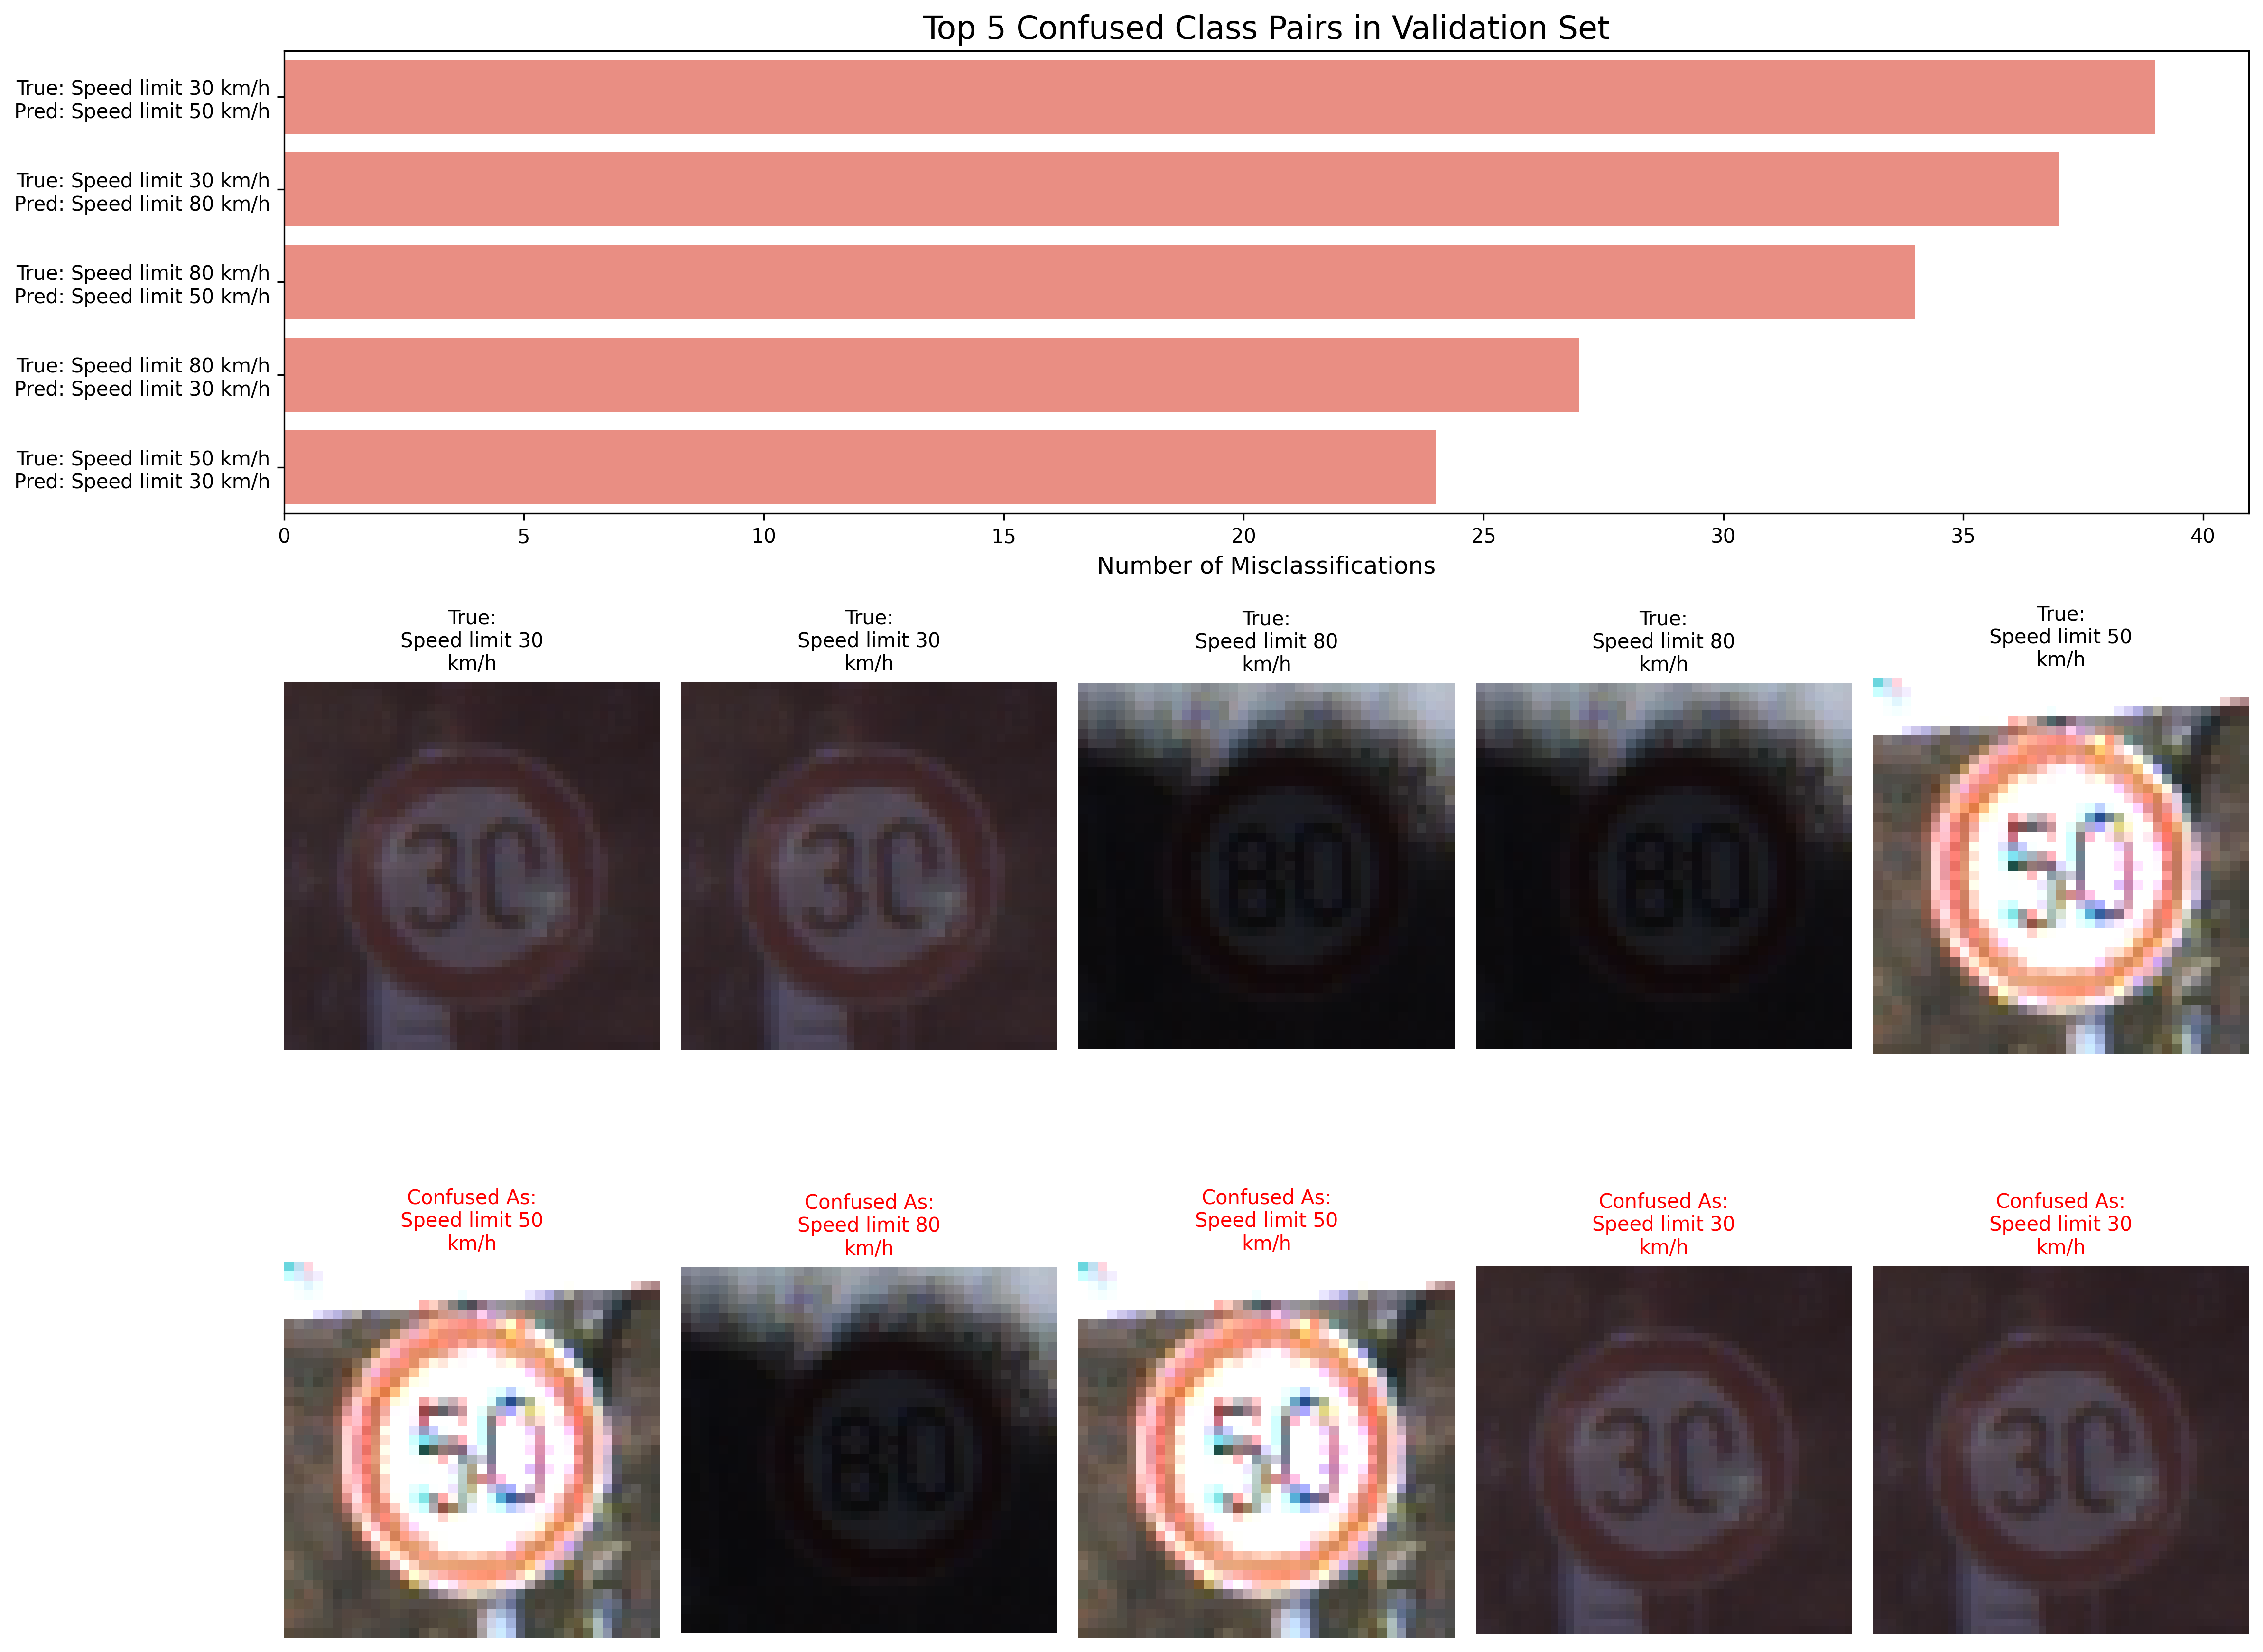
\includegraphics[width=\linewidth]{figures/enhanced/fig_08_error_analysis_v3.png}
    \caption{Detailed visualization of misclassified traffic signs and feature confusion.}
    \label{fig:error_analysis}
\end{figure}


% =========================
% 6. Conclusion
% =========================
\section{Conclusion}

By combining ROI-based preprocessing, HOG feature extraction, and a Linear Support Vector Machine, we established a lightweight yet effective pipeline for traffic sign recognition on the GTSRB dataset \cite{stallkamp2011gtsrb}. The 324-dimensional feature classifier successfully handles 43 sign categories with a 92.36\% validation accuracy, proving particularly robust on well-represented classes like "Priority road" and "Yield".

The fixed-size grid approach of HOG, however, struggles to capture subtle intra-class variations or overcome severe lighting and viewpoint distortions. This structural limitation directly causes misclassifications among underrepresented classes or signs sharing strong geometric similarities. 

To transcend these bottlenecks, subsequent research will pivot toward end-to-end representation learning. Adopting deep architectures—specifically Convolutional Neural Networks (CNNs) or Vision Transformers (ViTs)—would bypass manual feature engineering entirely, enabling the model to intrinsically learn hierarchical representations that are robust against adverse environmental conditions.

% =========================
\clearpage

% References
% =========================
\begingroup
\setlength{\parskip}{0pt}

\begin{thebibliography}{99}
\setlength{\itemsep}{0pt}

\bibitem{dalal2005hog}
N. Dalal and B. Triggs,
``Histograms of oriented gradients for human detection,''
in \emph{2005 IEEE Computer Society Conference on Computer Vision and Pattern Recognition (CVPR'05)}, 2005, pp. 886--893, doi: 10.1109/CVPR.2005.177.

\bibitem{boser1992svm}
B.~E. Boser, I.~M. Guyon, and V.~N. Vapnik,
``A training algorithm for optimal margin classifiers,''
in \emph{Proceedings of the Fifth Annual Workshop on Computational Learning Theory (COLT '92)}, 1992, pp. 144--152, doi: 10.1145/130385.130401.

\bibitem{lowe2004sift}
D.~G. Lowe,
``Distinctive image features from scale-invariant keypoints,''
\emph{International Journal of Computer Vision}, vol. 60, no. 2, pp. 91--110, 2004, doi: 10.1023/B:VISI.0000029664.99615.94.

\bibitem{neubeck2006nms}
A. Neubeck and L. Van Gool,
``Efficient non-maximum suppression,''
in \emph{18th International Conference on Pattern Recognition (ICPR 2006)}, 2006, pp. 850--855, doi: 10.1109/ICPR.2006.479.

\bibitem{lecun1998lenet}
Y. LeCun, L. Bottou, Y. Bengio, and P. Haffner,
``Gradient-based learning applied to document recognition,''
\emph{Proceedings of the IEEE}, vol. 86, no. 11, pp. 2278--2324, 1998, doi: 10.1109/5.726791.

\bibitem{ren2015faster}
S. Ren, K. He, R. Girshick, and J. Sun,
``Faster R-CNN: Towards Real-Time Object Detection with Region Proposal Networks,''
in \emph{Advances in Neural Information Processing Systems (NeurIPS)}, 2015, doi: 10.48550/arXiv.1506.01497.

\bibitem{liu2016ssd}
W. Liu et al.,
``SSD: Single Shot MultiBox Detector,''
in \emph{European Conference on Computer Vision (ECCV)}, 2016, pp. 21--37, doi: 10.1007/978-3-319-46448-0\_2.

\bibitem{redmon2016yolo}
J. Redmon, S. Divvala, R. Girshick, and A. Farhadi,
``You Only Look Once: Unified, Real-Time Object Detection,''
in \emph{2016 IEEE Conference on Computer Vision and Pattern Recognition (CVPR)}, 2016, pp. 779--788, doi: 10.1109/CVPR.2016.91.

\bibitem{lin2017retinanet}
T.-Y. Lin, P. Goyal, R. Girshick, K. He, and P. Doll\'{a}r,
``Focal loss for dense object detection,''
in \emph{2017 IEEE International Conference on Computer Vision (ICCV)}, 2017, doi: 10.1109/ICCV.2017.324.

\bibitem{mogelmose2012survey}
A. M{\o}gelmose, M.~M. Trivedi, and T.~B. Moeslund,
``Vision-based traffic sign detection and analysis for intelligent driver assistance systems: Perspectives and survey,''
\emph{IEEE Transactions on Intelligent Transportation Systems}, vol. 13, no. 4, pp. 1484--1497, 2012, doi: 10.1109/TITS.2012.2209421.

\bibitem{stallkamp2011gtsrb}
J. Stallkamp, M. Schlipsing, J. Salmen, and C. Igel,
``The German Traffic Sign Recognition Benchmark: A multi-class classification competition,''
in \emph{2011 International Joint Conference on Neural Networks}, 2011, pp. 1453--1460, doi: 10.1109/IJCNN.2011.6033395.

\bibitem{ertler2020mapillary}
C. Ertler, J. Jerneven, C. Kuo, H. Neuhold, P. Neuhold, and G. Ros,
``The Mapillary Traffic Sign Dataset for Detection and Classification on a Global Scale,''
in \emph{Proceedings of the European Conference on Computer Vision (ECCV)}, 2020, doi: 10.1007/978-3-030-58592-1\_5.

\bibitem{dosovitskiy2021vit}
A. Dosovitskiy et al.,
``An image is worth 16x16 words: Transformers for image recognition at scale,''
in \emph{International Conference on Learning Representations (ICLR)}, 2021, doi: 10.48550/arXiv.2010.11929.

% Keep key xing2025 to preserve existing \cite{xing2025}
\bibitem{xing2025}
Y. Jiang et al.,
``Multi-modal time series analysis: A tutorial and survey,''
in \emph{KDD}, 2025, pp. 6043--6053, doi: 10.1145/3711896.3736567.

% Keep key zhang2025 to preserve existing \cite{zhang2025}
\bibitem{zhang2025}
W. Xu et al.,
``FinMultiTime: A four-modal bilingual dataset for financial time-series analysis,''
\emph{arXiv preprint arXiv:2506.05019}, 2025.

\end{thebibliography}
\endgroup

\end{document}